% utf-8 ru, unix eolns
\documentclass[12pt,a4paper,oneside]{extarticle}
    \righthyphenmin=2 %минимально переносится 2 символа %%%
    \sloppy

% Рукопись оформлена в соответствии с правилами оформления 
% электронной версии авторского оригинала, 
% принятыми в Издательстве МГТУ им. Н.Э. Баумана.

\usepackage{geometry} % А4, примерно 28-31 строк(а) на странице 
    \geometry{paper=a4paper}
    \geometry{includehead=false} % Нет верх. колонтитула
    \geometry{includefoot=true}  % Есть номер страницы
    \geometry{bindingoffset=0mm} % Переплет    : 0  мм
    \geometry{top=20mm}          % Поле верхнее: 20 мм
    \geometry{bottom=25mm}       % Поле нижнее : 25 мм 
    \geometry{left=25mm}         % Поле левое  : 25 мм
    \geometry{right=25mm}        % Поле правое : 25 мм
    \geometry{headsep=10mm}  % От края до верх. колонтитула: 10 мм
    \geometry{footskip=20mm} % От края до нижн. колонтитула: 20 мм 

\usepackage{cmap}
\usepackage[T2A]{fontenc} 
\usepackage[utf8x]{inputenc}
\usepackage[english,russian]{babel}
\usepackage{misccorr}

\usepackage{amsmath}
\usepackage{amsfonts}
\usepackage{amssymb}

%\usepackage{cm-super} %человеческий рендер русских шрифтов

\setlength{\parindent}{1.25cm}  % Абзацный отступ: 1,25 см
\usepackage{indentfirst}        % 1-й абзац имеет отступ

\usepackage{setspace}   

\onehalfspacing % Полуторный интервал между строками

\makeatletter
\renewcommand{\@oddfoot }{\hfil\thepage\hfil} % Номер стр.
\renewcommand{\@evenfoot}{\hfil\thepage\hfil} % Номер стр.
\renewcommand{\@oddhead }{} % Нет верх. колонтитула
\renewcommand{\@evenhead}{} % Нет верх. колонтитула
\makeatother

\usepackage{fancyvrb}


\usepackage[pdftex]{graphicx}  % поддержка картинок для пдф
\graphicspath{ {./pictures/} }
\usepackage{rotating}
%\DeclareGraphicsExtensions{.jpg,.png}




\renewcommand{\labelenumi}{\theenumi.} %меняет вид нумерованного списка

\usepackage{perpage} %нумерация сносок 
\MakePerPage{footnote}

\usepackage[all]{xy} %поддержка графов

\usepackage{listings} %листинги


\usepackage{url}


\usepackage{tikz} %для рисования графиков
\usepackage{pgfplots}

\usepackage{gensymb}

\usepackage{ccaption}%изменяет подпись к рисунку
\makeatletter 
\renewcommand{\fnum@figure}[1]{Рисунок~\thefigure~---~\sffamily}
\makeatother

\begin{document}
\pgfplotsset{compat=1.8}

\thispagestyle{empty}
\newpage
{
\centering


\textbf{
МОСКОВСКИЙ ГОСУДАРСТВЕННЫЙ ТЕХНИЧЕСКИЙ УНИВЕРСИТЕТ ИМЕНИ Н. Э. БАУМАНА \\
Факультет информатики и систем управления \\
Кафедра теоретической информатики и компьютерных технологий}
\bigskip
\bigskip
\bigskip
\bigskip
\bigskip
\bigskip
\bigskip

\vfill


Лабораторная работа №4 \\
по курсу <<Моделирование>>

\bigskip

{\large <<Построение разрезов поверхностей>>}
\bigskip

\vfill



\hfill\parbox{4cm} {
Выполнил:\\
студент ИУ9-111 \hfill \\
Выборнов А. И.\hfill \medskip\\
Руководитель:\\
Домрачева А. Б.\hfill
}


\vspace{\fill}

Москва \number\year
\clearpage
}



\clearpage


\section{Постановка задачи}
    Одной из базовых задач анализа триангуляционных поверхностей является построение разрезов --- вертикальных (профилей) и горизонтальных (изолиний).

    {\it Изолиниями} уровня $h$ называют геометрическое место точек на поверхности, имеющих высоту $h$ и имеющих в любой своей окрестности другие точки с меньшей высотой:
    $I_h = \{(x,y) | z(x,y)=h, \forall \epsilon > 0 \colon \exists (x',y') \colon |(x',y'),(x,y)|<\epsilon, z(x',y')<h \}$.

    {\it Изоконтурами} между уровнями $h_1$ и $h_2$ называют замыкание геометрического места точек на поверхности, имеющих высоту $h \in [h_1, h_2)$, т.е. множество точек $I_h~=~\overline{\{ (x, y) | h_1 <= z(x,y) < h_2 \}}$.

    В задаче построения изоконтуров требуется построить множество непересекающихся регионов, каждый из которых представляет область, высоты точек внутри которой лежат в определенном диапазоне. Обычно задаётся система диапазонов с помощью начального значения самого первого диапазона, конечного значения последнего диапазона и шага построения диапазонов.

    По трёхмерной модели поверхности нужно построить множество изоконтуров, лежащих в диапазоне $[h_1, h_2)$ с шагом $\Delta h$.

\section{Теоретическая часть}
    \subsection{Построение изолиний}
        Для построения изолиний высотой h используется следующий алгоритм:

        \begin{enumerate}
            \item Помечаем каждый треугольник триангуляции, по которому проходят изолинии (т.е. выполняется условие $min( z_1, z_2, z_3 ) < h < < max( z_1, z_2, z_3 )$, где $z_i$ --- высоты трех его вершин), флагом $C_i := 1$ , а все остальные треугольники – $C_i := 0$. Если обнаружен хотя бы один треугольник, у которого хотя бы одно ребро лежит в плоскости изолинии, то $h$ уменьшается на некоторое малое $\Delta h$ и алгоритм повторяется заново.
            \item  Для каждого треугольника с $C_i = 1$ выполняем отслеживание очередной изолинии в обе стороны от данного треугольника, пока один конец не выйдет на другой или на границу триангуляции. Каждый пройденный при отслеживании треугольник помечается $C_i := 0$ . Конец алгоритма.
        \end{enumerate}

        Трудоемкость такого алгоритма, очевидно, является линейной относительно размера триангуляции.

    \subsection{Построение изоконтуров}
        Для построения множества изоконтуров, лежащих в диапазоне $[h_1, h_M)$ с шагом $\Delta h$ используется следующий алгоритм:
         \begin{enumerate}
            \item Пусть заданы уровни $h_1 ,..., h_M$, Обнуляем множества ломаных, входящих в изоконтуры: $C_i = \varnothing, i = \overline{0, M}$.
            \item Для каждого уровня $h_i$ строим изолинии. Каждую замкнутую изолинию добавляем во множество $C_i$ .
            \item Определяем все кусочки границы триангуляции между точками выхода изолиний на границу. Формируем граф, в котором в качестве узлов выступают точки выхода на границу, а в качестве рёбер --- кусочки границы между этими точками и рассчитанные изолинии. Каждая изолиния должна войти в граф дважды в виде одинаковых ориентированных рёбер, но направленных в разные стороны. Для рёбер ---кусочков границы --- устанавливаем такую ориентацию, чтобы внутренности триангуляции находились справа по ходу движения. В результате в каждом узле графа должны сходиться четыре ребра.
            \item По полученному графу строим контуры. Начинаем движение с любой вершины графа и двигаемся вперед в соответствии с ориентацией рёбер до тех пор, пока не вернемся в начальную вершину. Повторный проход по одному и тому же ребру запрещен, для чего делаются специальные пометки на рёбрах. При попадании в узел графа из граничной цепочки далее надо двигаться по ребру, cоответствующему изолинии, иначе --- по граничному ребру. Обратим внимание, что каждая изолиния войдет в два контура, соответствующих разным диапазонам высот.
            \item Для каждого полученного на предыдущем шаге контура определяем, какому диапазону высот он соответствует. Для этого нужно взять и проверить любое ребро триангуляции, входящее в составе граничной цепочки, использованной в каждом контуре. На основании этого помещаем цепочку в соответствующее множество $C_i$. Конец алгоритма.
        \end{enumerate}

        Трудоемкость данного алгоритма линейно зависит от размера триангуляции и количества изолиний.
        
\section{Реализация}
    В рамках лабораторной работы была написана программа на языке python, её разработка производилась в несколько этапов:

    \begin{enumerate}
        \item Получение и хранение триангулированной модели объекта. 
        \item Считывание модели в оперативную память.
        \item Построение изолинии.
        \item Построение изоконтуров.
        \item Визуализация результатов.
    \end{enumerate}
%\clearpage
    \subsection{Получение и хранение триангулированной модели объекта}
        Для построения трёхмерного объекта и его триангулированной модели был использован пакет {\it Blender} --- свободный, профессиональный пакет для создания трёхмерной компьютерной графики, включающий в себя средства моделирования, анимации, рендеринга, постобработки и монтажа видео со звуком, а также для создания интерактивных игр. На рисунке \ref{pic:blender} показан скриншот работы по созданию модели с помощью blender.

        \begin{figure}[h!]
            \center
            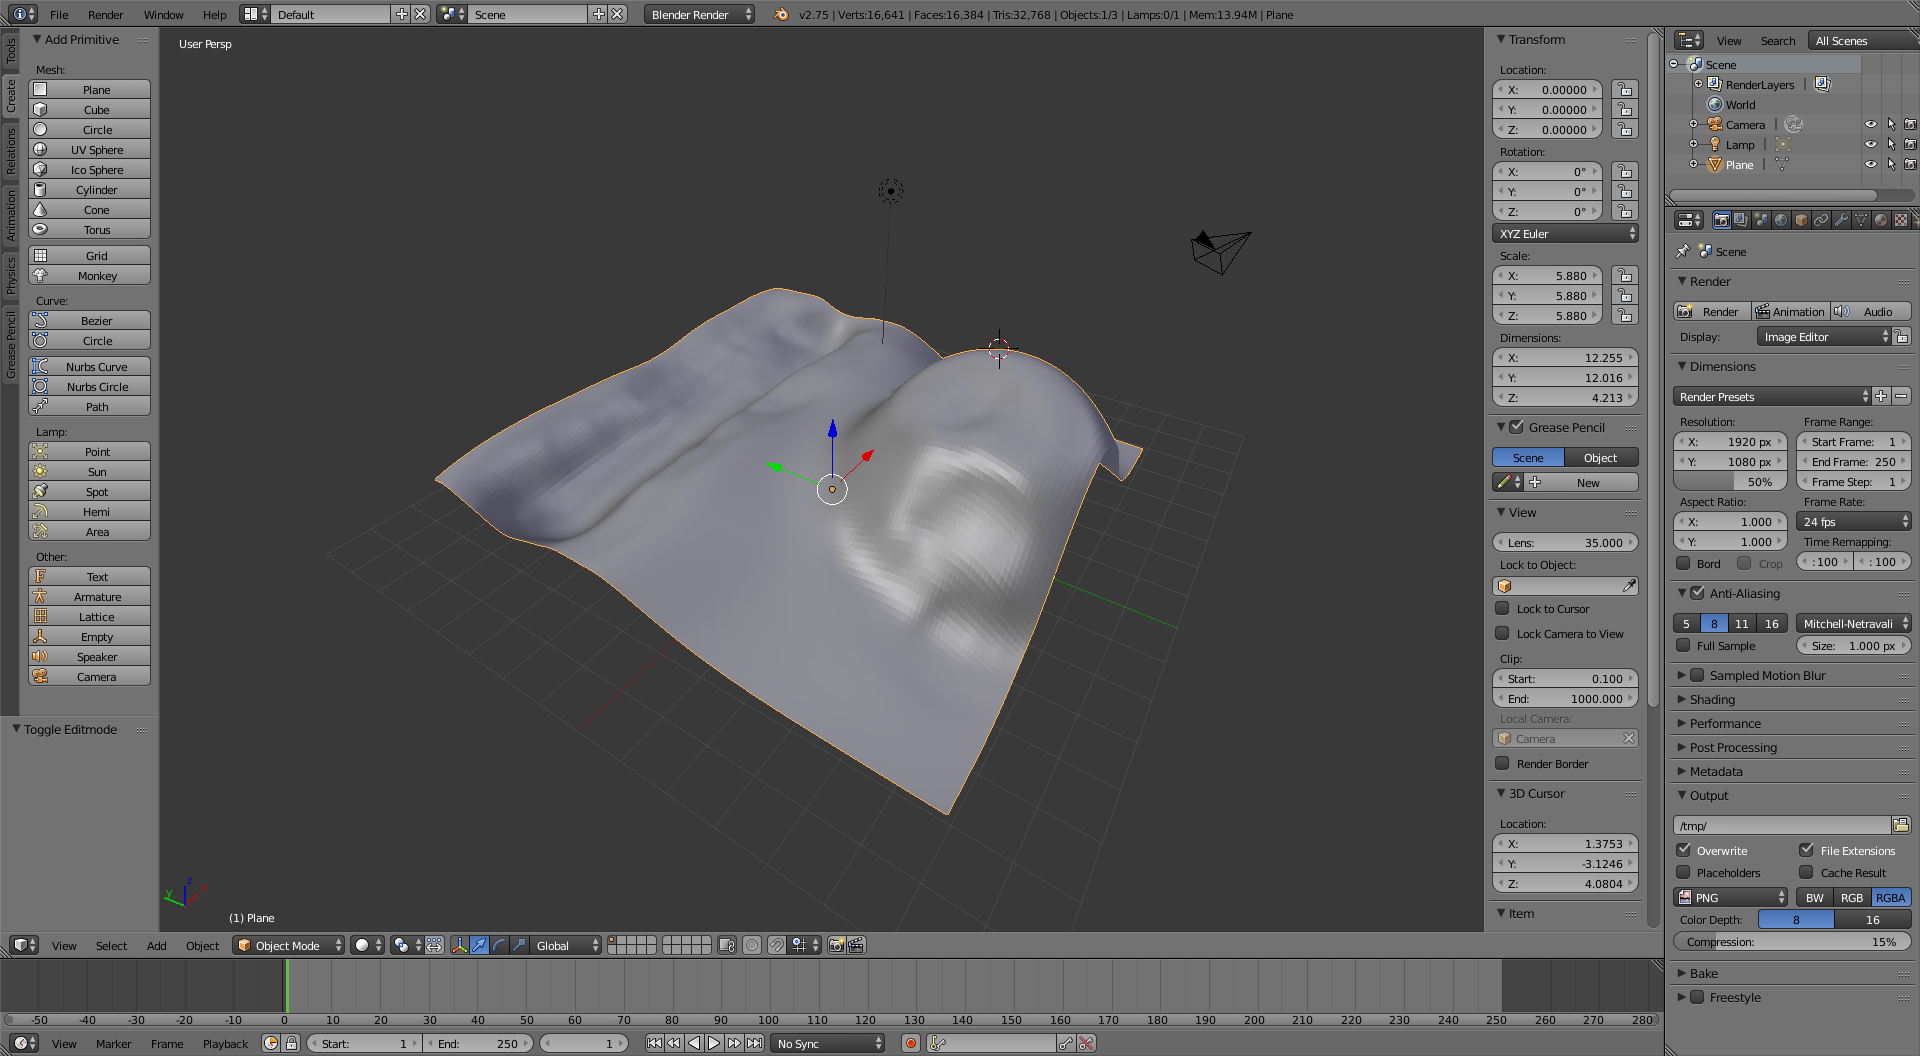
\includegraphics[scale=0.2]{blender.png}
            \caption{Скриншот работы по созданию модели в blender.}
            \label{pic:blender}
        \end{figure}

        
        {\it OBJ} --- это простой формат данных, который содержит только геометрию, а именно, позицию каждой вершины, связь координат текстуры с вершиной, нормаль для каждой вершины, а также параметры, которые создают полигоны. Данный формат был выбран из-за простоты, человекочитаемости человеком, а также поддержки этого формата всеми основными графическими редакторами.

    \subsection{Считывание модели в оперативную память}
        Программа получает на вход файл в OBJ формате. Затем она считывает из него информацию о координатах каждой вершины и о полигонах~(в рамках этой работы все полигоны треугольные), которые связывают эти вершины.

        В программе эта информация описывается с помощью трёх классов: Triangle~(соответствует треугольному полигону), Edge~(соответствует ребру) и Vertex~(соответствует вершине).
        \begin{itemize}
            \item Triangle --- класс, описывающий треугольный полигон. Этот класс содержит информацию о трёх рёбрах, его составляющих.
            \item Edge --- класс, описывающий отрезок, представляющий собой грань полигона. Содержит информацию о вершинах его составляющих, а также о треугольниках, ребром которых он является. Для каждого ребра существует только один экземпляр класса Edge, это обеспечивается с помощью образца проектирования Фабрика~(Factory), который возвращает новое ребро, если оно ещё не было создано, иначе возвращает уже существующий экземпляр класса.
            \item Vertex --- класс, описывающий вершину. Хранит информацию о координатах этой вершины в трёхмерном пространстве и о рёбрах, в которые эта вершина входит.
        \end{itemize}
    \clearpage    
    \subsection{Построение изолинии}
        Построение изолинии выполнялось согласно алгоритму описанному в теоритической части. В итоге по модели мы получаем список изолиний, с отметками являются ли они замкнутыми. Пример получающихся изолинию приведён на рисунке~\ref{pic:isoline}.

        \begin{figure}[h!]
            \center
            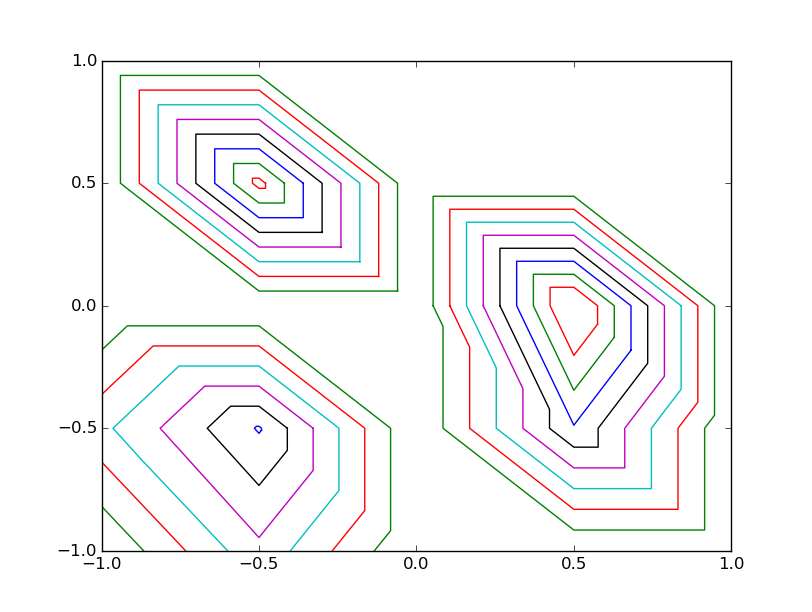
\includegraphics[scale=0.7]{isoline.png}
            \caption{Изолинии.}
            \label{pic:isoline}
        \end{figure}

    \subsection{Построение изоконтурова}
        Для замкнутых изолиний получение изоконтура тривиально --- помещаем изолинию в множество, соответствующее её высоте, а для незамкнутых построение происходит в два этапа:

        \begin{enumerate}
            \item Формирование графа, содержащего точки выхода на границу изолиний и вершины всех граничных рёбер.
            \item Построение по графу контуров.
        \end{enumerate}

        При реализации строился граф, немного отличный от описанного в теоретической части.
        По причине того, что описанный в теоретической части граф достаточно сложно получить.
        Опишем используемый граф, с помощью алгоритма его построения:

        \begin{enumerate}
            \item Добавим в граф в качестве вершин точки выхода изолиний на границу.
            Каждую изолиню добавим в виде двух рёбер направленных в разные стороны, которые соединяют соответствующие изолинии вершины. Во время добавления вершин, запомним для каждого граничного ребра, какие изолинии их пересекают.
            \item Для каждого граничного ребра модели выполним следующий алгоритм:
            \begin{enumerate}
                \item Если ребро не пересекается изолиниями, то добавим в граф в качестве вершин, его узлы и соединим их ребром графа, направленным так, чтобы внутренность треугольника осталась справа (проверка выполняется с помощью векторного произведения).
                \item Иначе разобьём ребра на множество последовательных не пересекающихся отрезков, вершинами которых являются узлы ребра и точки пересечения изолиний с этим ребром. Каждый отрезок добавим в граф, аналогично ребру, не пересекаемому изолиниями.
            \end{enumerate}
        \end{enumerate}

        Граф в программе представлен в виде трёх классов:
        \begin{itemize}
            \item Graph --- класс, хранящий граф в формате отображения вершины графа в множество пар (ребро, вершина). Каждый элемент множества соответсвует исходящему из исходной вершины рёбру и вершине, куда это ребро ведёт.
            \item GraphEdge --- класс, описывающий ребро графа. Содержит информацию о изолинии, если она в нём содержится.
            \item GraphNode --- класс, описывающий вершину графа. Хранит в себе экземпляр класса Vertex. Для каждой вершины существует только один экземпляр класса GraphNode, это обеспечивается с помощью образца проектирования Фабрика.
        \end{itemize}

        Пример получаемоего графа приведён на рисунке~\ref{pic:graph}. Вершины обозначены овалами с координатами, рёбра обозначены стрелками с подписями: border --- ребра соответствующее участку границы, isoline --- ребро соответствующее изолинии. Все вершины графа расположены в пространстве в соответствии с их координатами на двумерной плоскоти $x0y$.

        \begin{figure}[h!]
            \center
            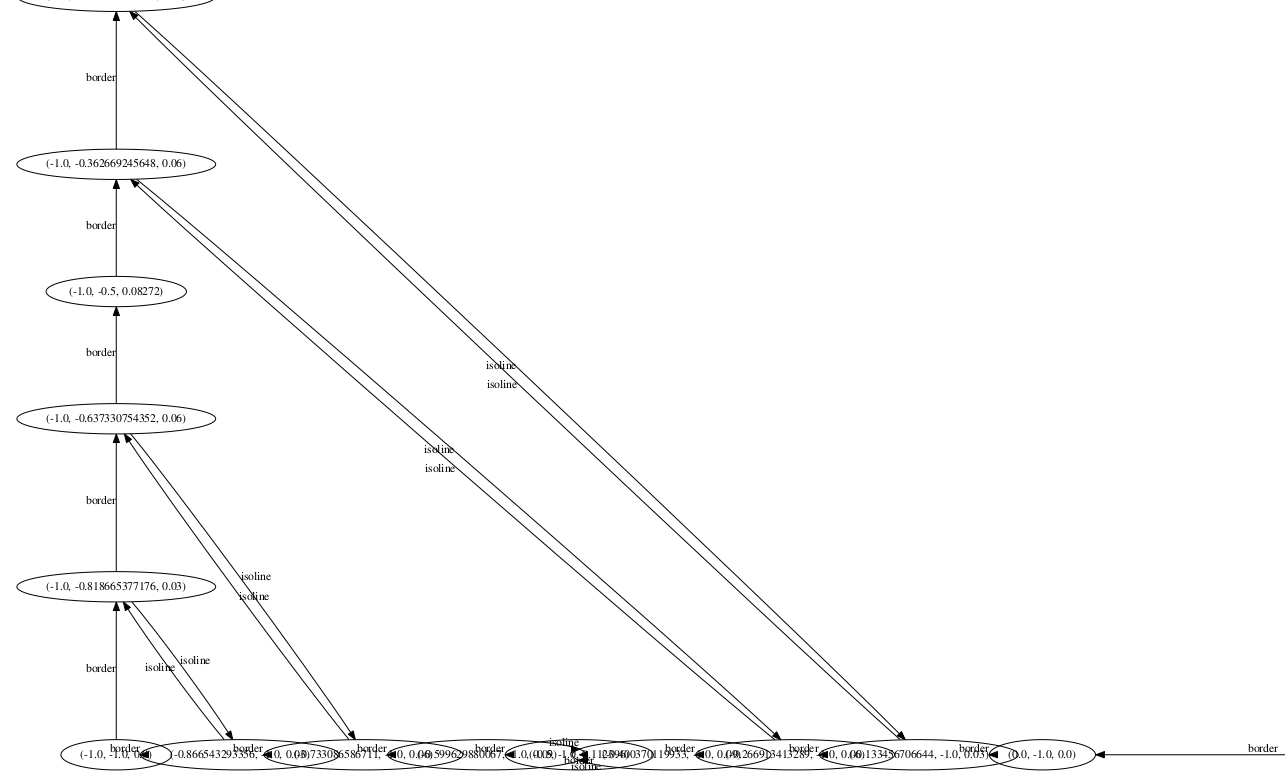
\includegraphics[scale=0.3]{graph.png}
            \caption{Граф, используемый при построении изоконтуров.}
            \label{pic:graph}
        \end{figure}

        Для получения по графу изоконтура, выполняем обход графа, который начинается с любой вершины. Обход заключается в проходе по рёбрам графа согласно их направлениям, до тех пор пока не вернёмся в исходную вершину. При этом если мы прошли по изолинии, то в следующий раз мы обязательно должны пройти по ребру модели. А если мы прошли по ребру модели и перед нами стоит выбор идти далее по изолии или ребру - всегда выбираем изолинию. В результате получаем изоконтур, которые соотносим с высотой, соответствующей наиболее низкой изолинии, входящей в этот контур. Пример контура, который мы получаем после обхода можно увидеть на рисунке~\ref{pic:contour}.

        \begin{figure}[h!]
            \center
            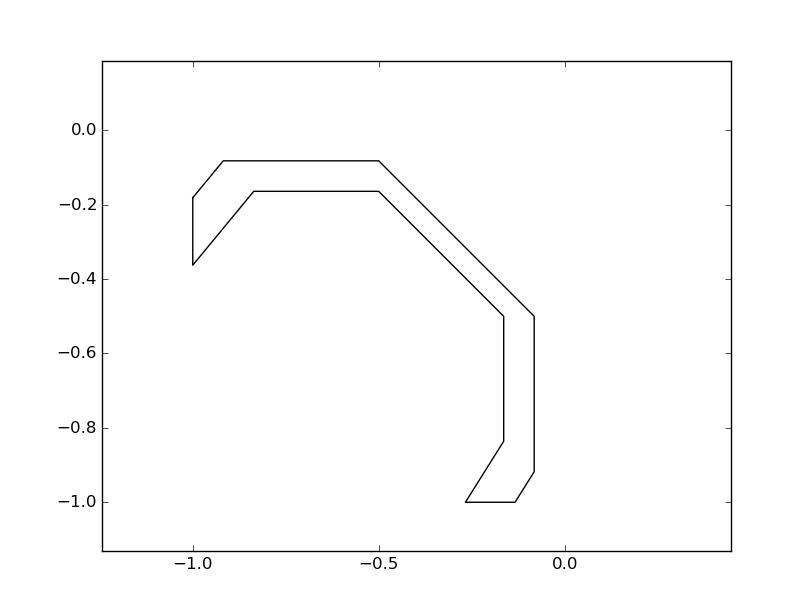
\includegraphics[scale=0.5]{contour.png}
            \caption{Изоконтур, который получился из незамкнутой изолинии.}
            \label{pic:contour}
        \end{figure}

    \subsection{Визуализация результатов}
        Визуализация изолиний и изоконтуров выполняется с помощью matplotlib --- библиотека на языке программирования Python для визуализации данных. Визуализация графа выполняется с помощью порождения файла на языке DOT, с последующей визуализацией с помощью graphviz --- пакета утилит по автоматической визуализации графов, заданных в виде описания на языке DOT.

        Результатом работы программы является изображение изоконтуров. Изображение получается с помощью последовательного рисования раскрашенных фигур, соответствующих изоконтурам. Изоконтуры рисуются последовательно~(начиная с самого нижнего, заканчивая самым верхним), друг поверх друга. При этом с увеличением высоты пропорционально изменяется цвет заливки от светло-серого то тёмно-серого. Пример изображения, получаемого в результате работы программы, показан на рисунке~\ref{pic:result}.
        
        \begin{figure}[h!]
            \center
            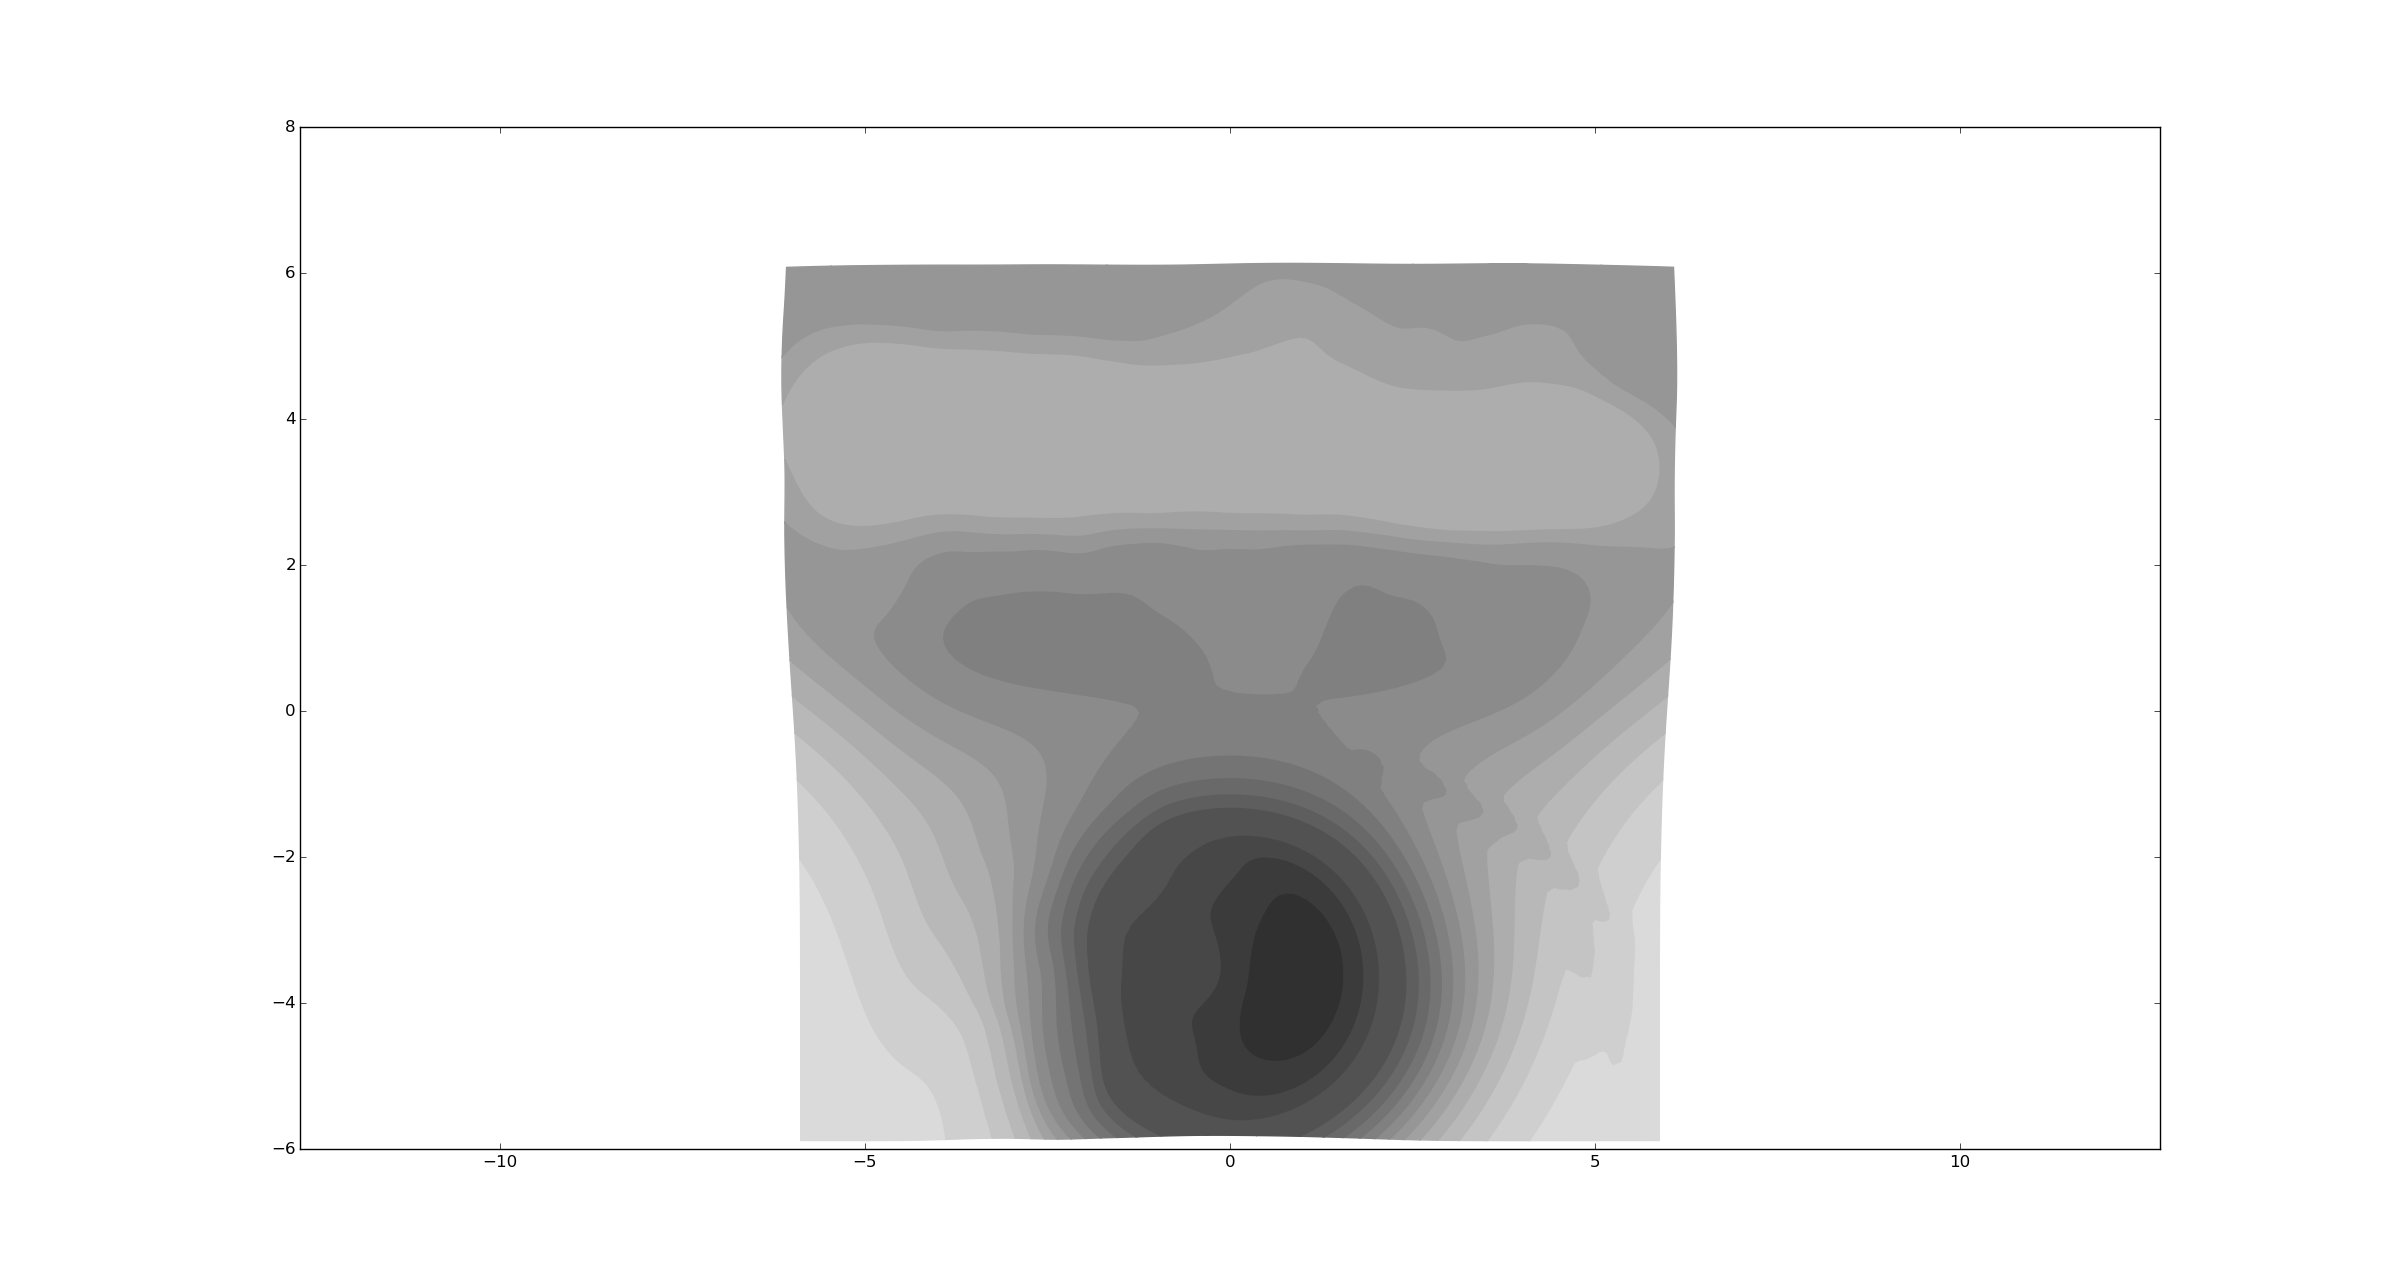
\includegraphics[scale=0.25]{result.png}
            \caption{Визуализация результата работы программы.}
            \label{pic:result}
        \end{figure}
\clearpage

\section{Тестирование}
    Для тестирования были использованы две модели: модель 1, состоящая из 32 полигонов, изображена на рисунке~\ref{pic:mini}, и модель 2, состоящая из 32768 полигонов, изображена на рисунке~\ref{pic:big}.
    \begin{figure}[h!]
            \center
            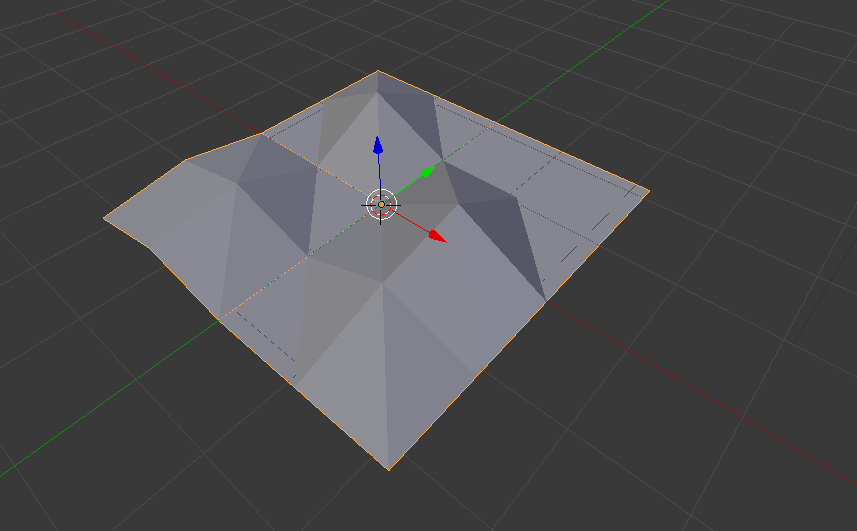
\includegraphics[scale=0.4]{mini.png}
            \caption{Модель 1, состоящая из 32 полигонов.}
            \label{pic:mini}
    \end{figure}

    \begin{figure}[h!]
            \center
            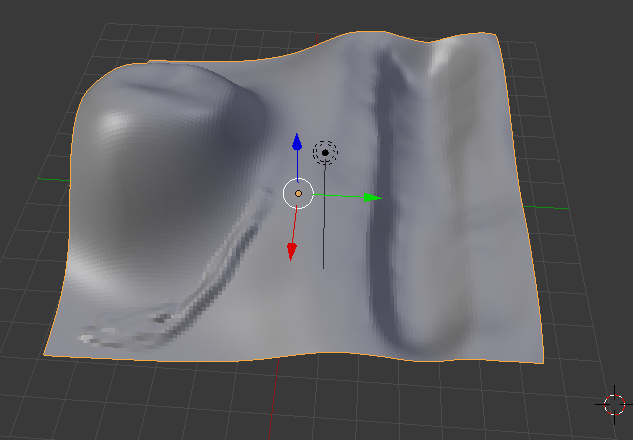
\includegraphics[scale=0.5]{big.png}
            \caption{Модель 2, состоящая из 32768 полигонов.}
            \label{pic:big}
    \end{figure}
    
    Результаты работы программы в зависимости от входных параметров приведены в таблице~\ref{tabular:results}. Из результатов видно, что больший шаг соответствует менее подробному разрезу и меньшему времени работы.

    \begin{table}[ht!]
                  
        \caption{Результаты работы программы в зависимости от входных параметров. \bigskip}
        \centering             
        
        \label{tabular:results}  
        %\begin{adjustbox}{angle=90}
        \begin{sideways}
        \begin{tabular}{|l|l|l|l|l|l|}
            \hline
            \textbf{Название модели} & \textbf{Нижняя граница} & \textbf{Верхняя граница} & \textbf{Шаг} & \textbf{Время работы (секунды)} & \textbf{Рисунок с результатом}
            \\ \hline
            Модель 1 & 0 & 0.25 & 0.01 & 0.513 & Рисунок~\ref{pic:mini1}
            \\ \hline
            Модель 1 & 0 & 0.25 & 0.03 & 0.440 & Рисунок~\ref{pic:mini2}
            \\ \hline
            Модель 1 & 0 & 0.25 & 0.05 & 0.413 & Рисунок~\ref{pic:mini3}
            \\ \hline

            Модель 2 & 0 & 4.25 & 0.1 & 13.312 & Рисунок~\ref{pic:big1}
            \\ \hline
            Модель 2 & 0 & 4.25 & 0.25 & 6.670 & Рисунок~\ref{pic:big2}
            \\ \hline
            Модель 2 & 0 & 4.25 & 0.5 & 4.116 & Рисунок~\ref{pic:big3}
            \\ \hline
        \end{tabular}   
        \end{sideways}     

    \end{table}

    \begin{figure}[h!]
        \center
        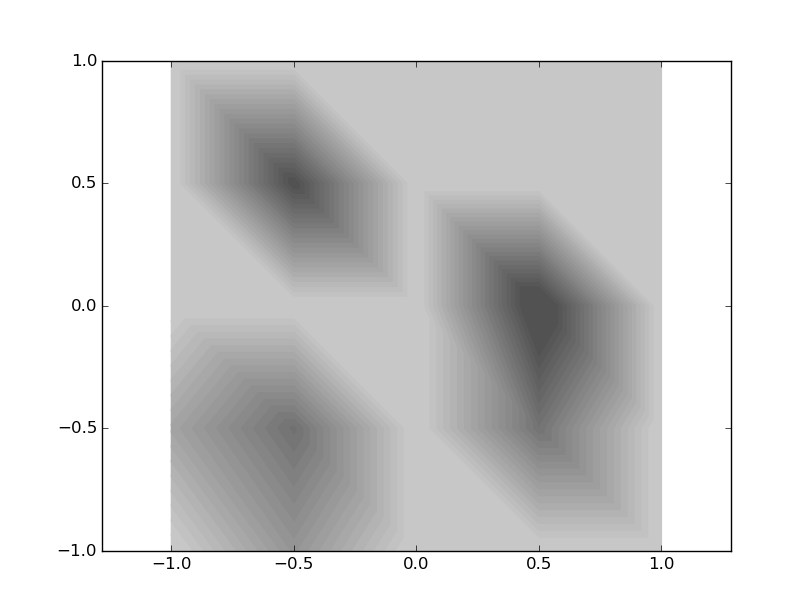
\includegraphics[scale=0.5]{mini1.png}
        \caption{Результат работы программы. Модель 1, нижняя граница 0, верхняя граница 0.25, шаг 0.01.}
        \label{pic:mini1}
    \end{figure}

    \begin{figure}[h!]
        \center
        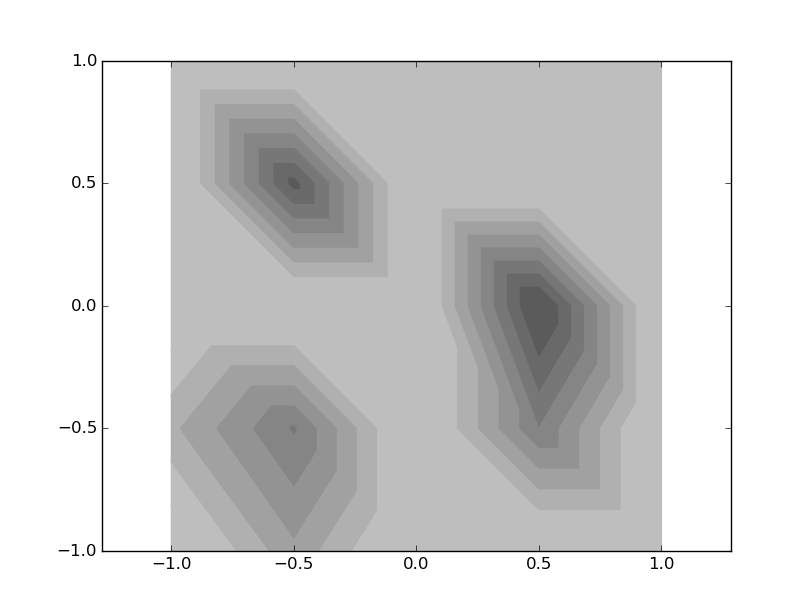
\includegraphics[scale=0.5]{mini2.png}
        \caption{Результат работы программы. Модель 1, нижняя граница 0, верхняя граница 0.25, шаг 0.03.}
        \label{pic:mini2}
    \end{figure}

    \begin{figure}[h!]
        \center
        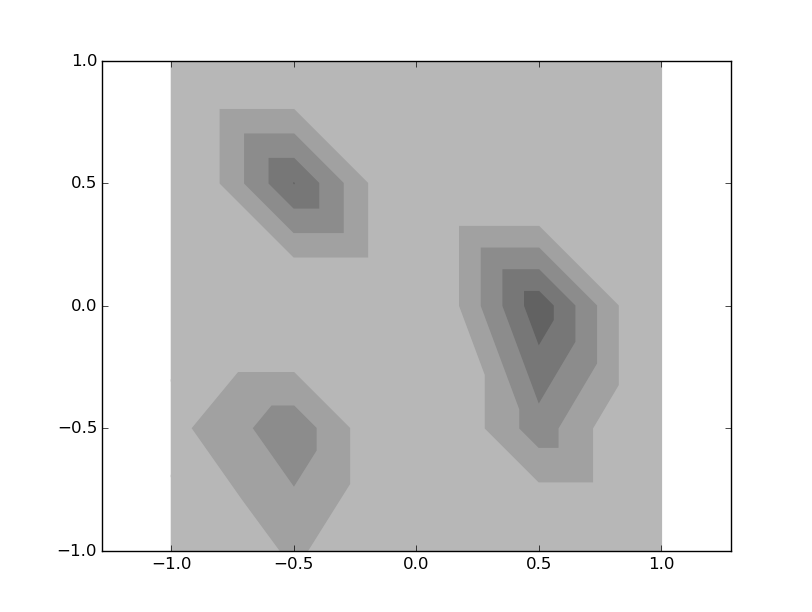
\includegraphics[scale=0.5]{mini3.png}
        \caption{Результат работы программы. Модель 1, нижняя граница 0, верхняя граница 0.25, шаг 0.05.}
        \label{pic:mini3}
    \end{figure}

    \begin{figure}[h!]
        \center
        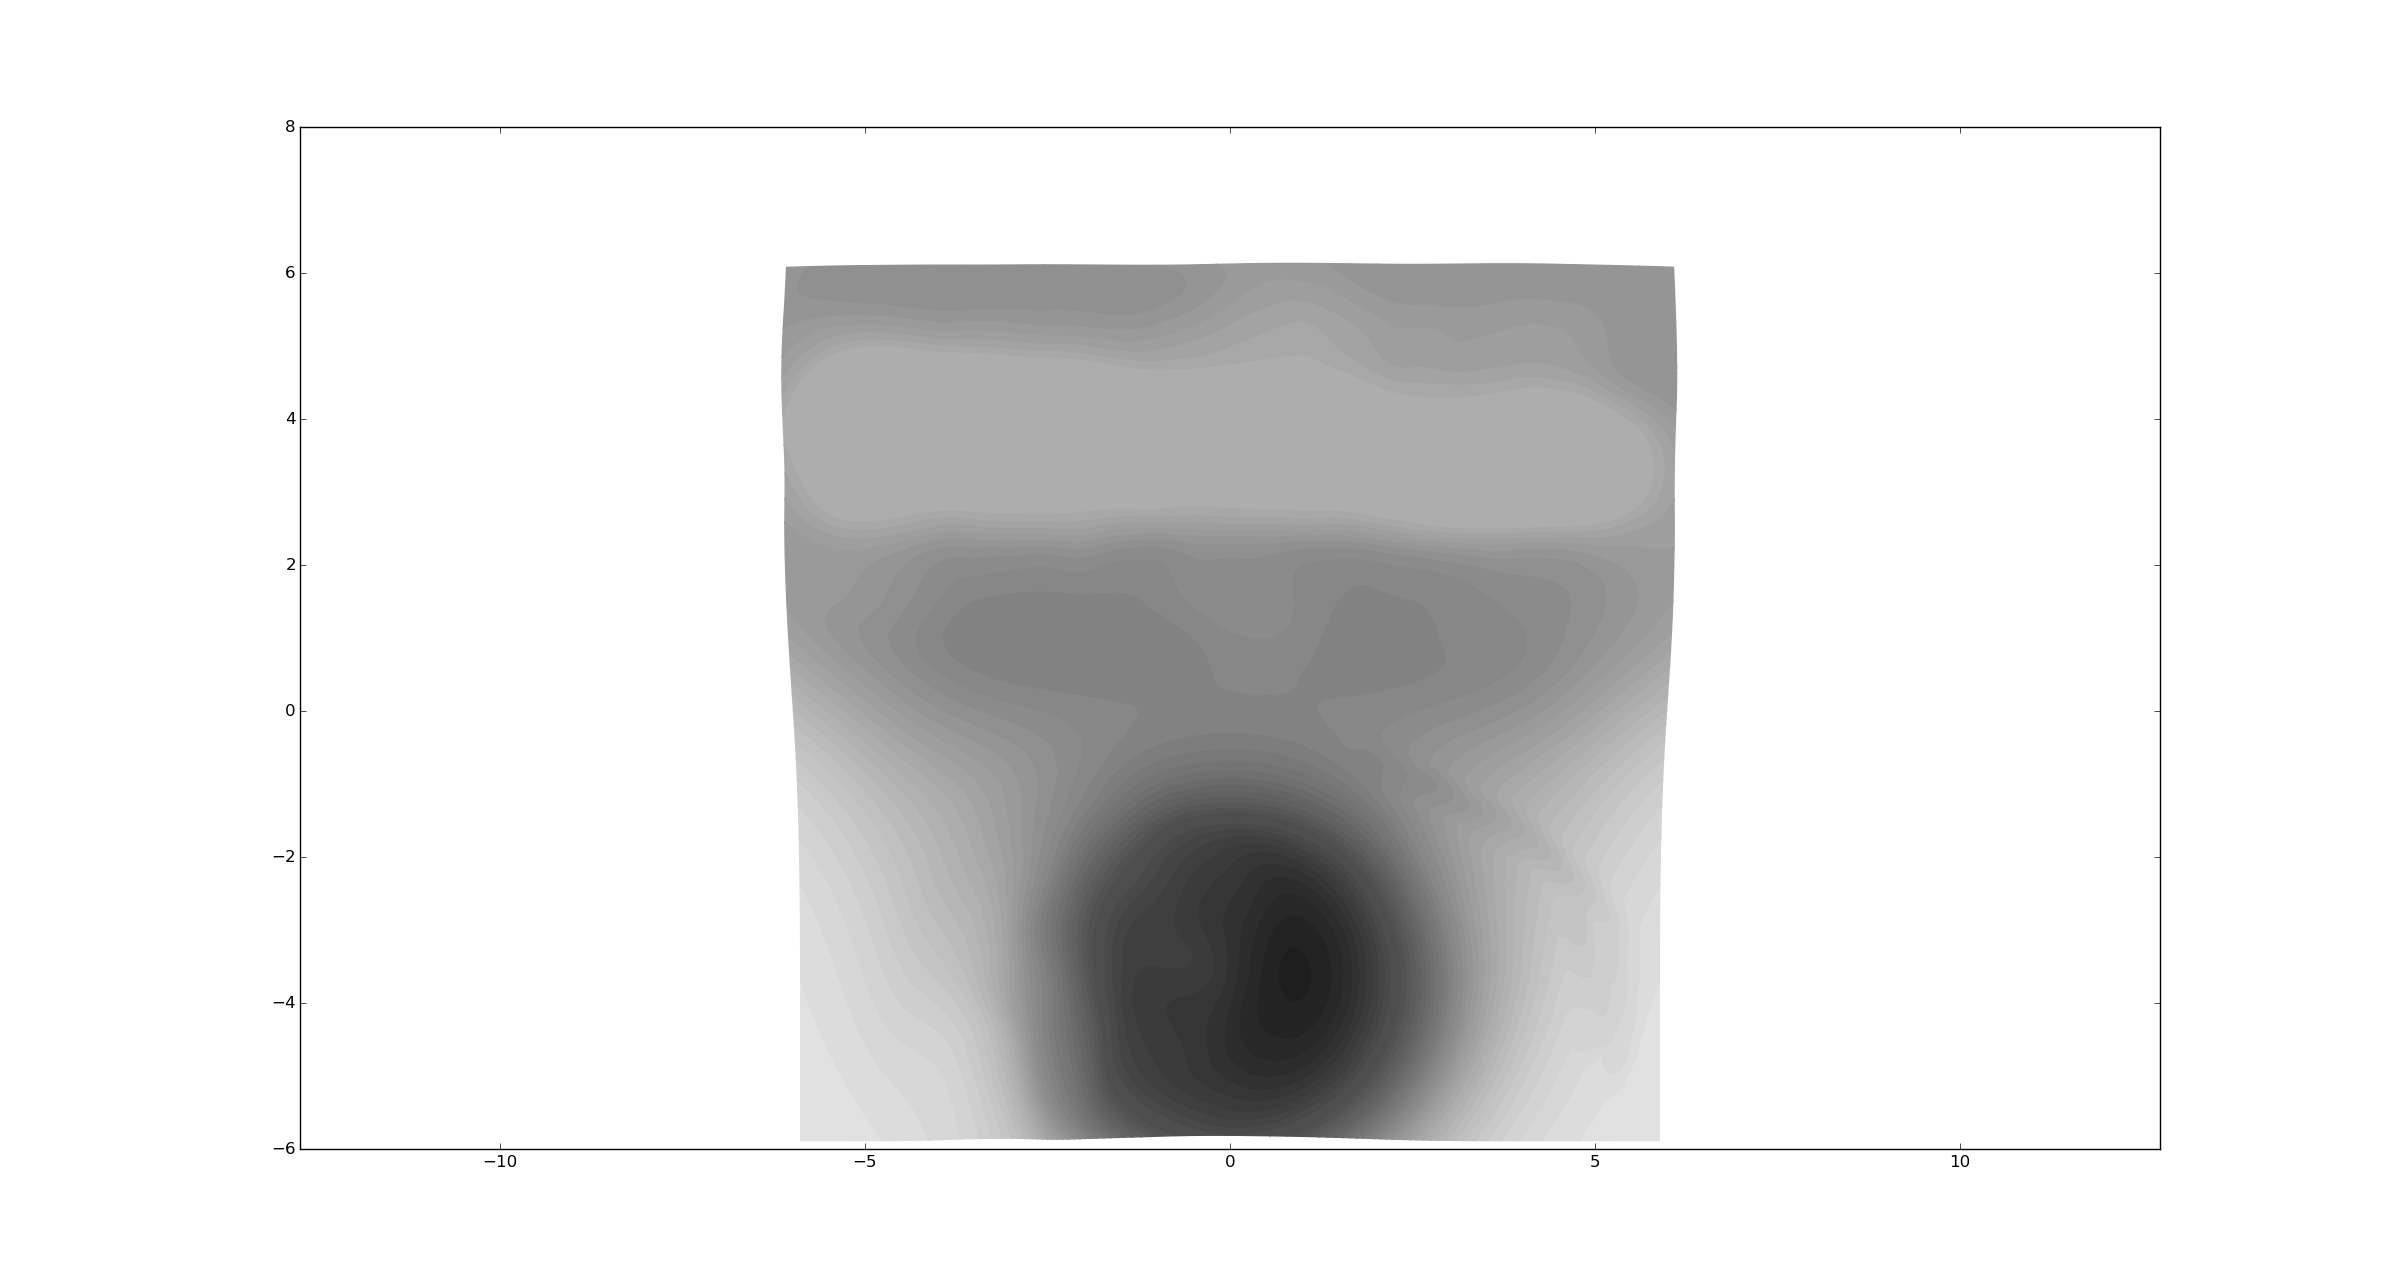
\includegraphics[scale=0.25]{big1.png}
        \caption{Результат работы программы. Модель 2, нижняя граница 0, верхняя граница 4.25, шаг 0.1.}
        \label{pic:big1}
    \end{figure}

    \begin{figure}[h!]
        \center
        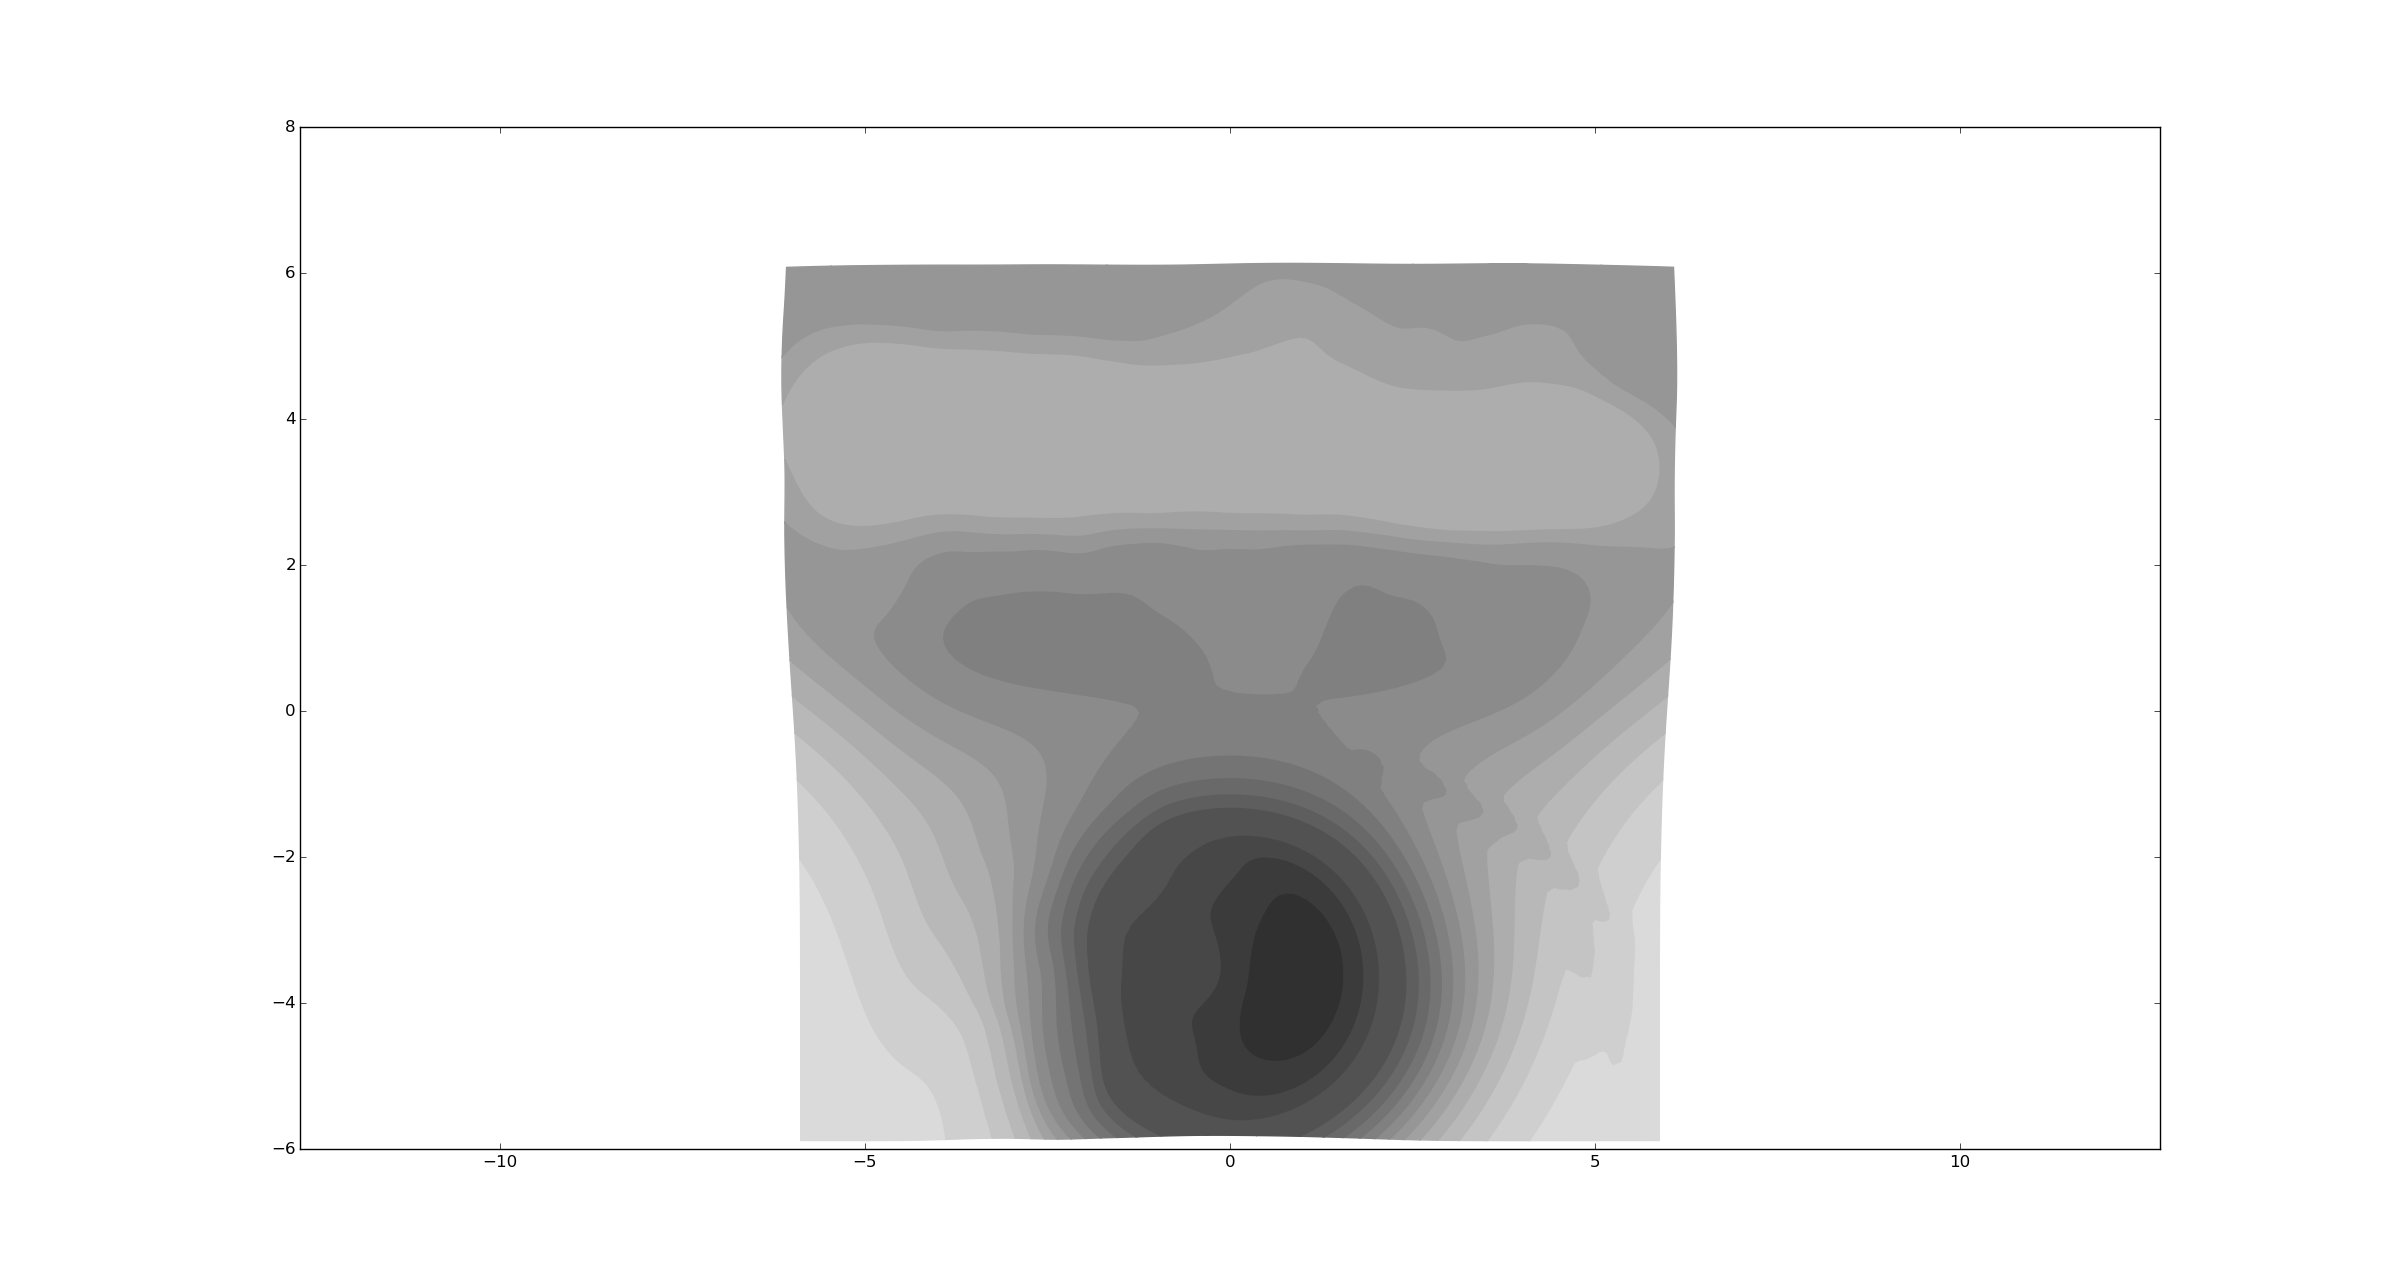
\includegraphics[scale=0.25]{big2.png}
        \caption{Результат работы программы. Модель 2, нижняя граница 0, верхняя граница 4.25, шаг 0.25.}
        \label{pic:big2}
    \end{figure}

    \begin{figure}[h!]
        \center
        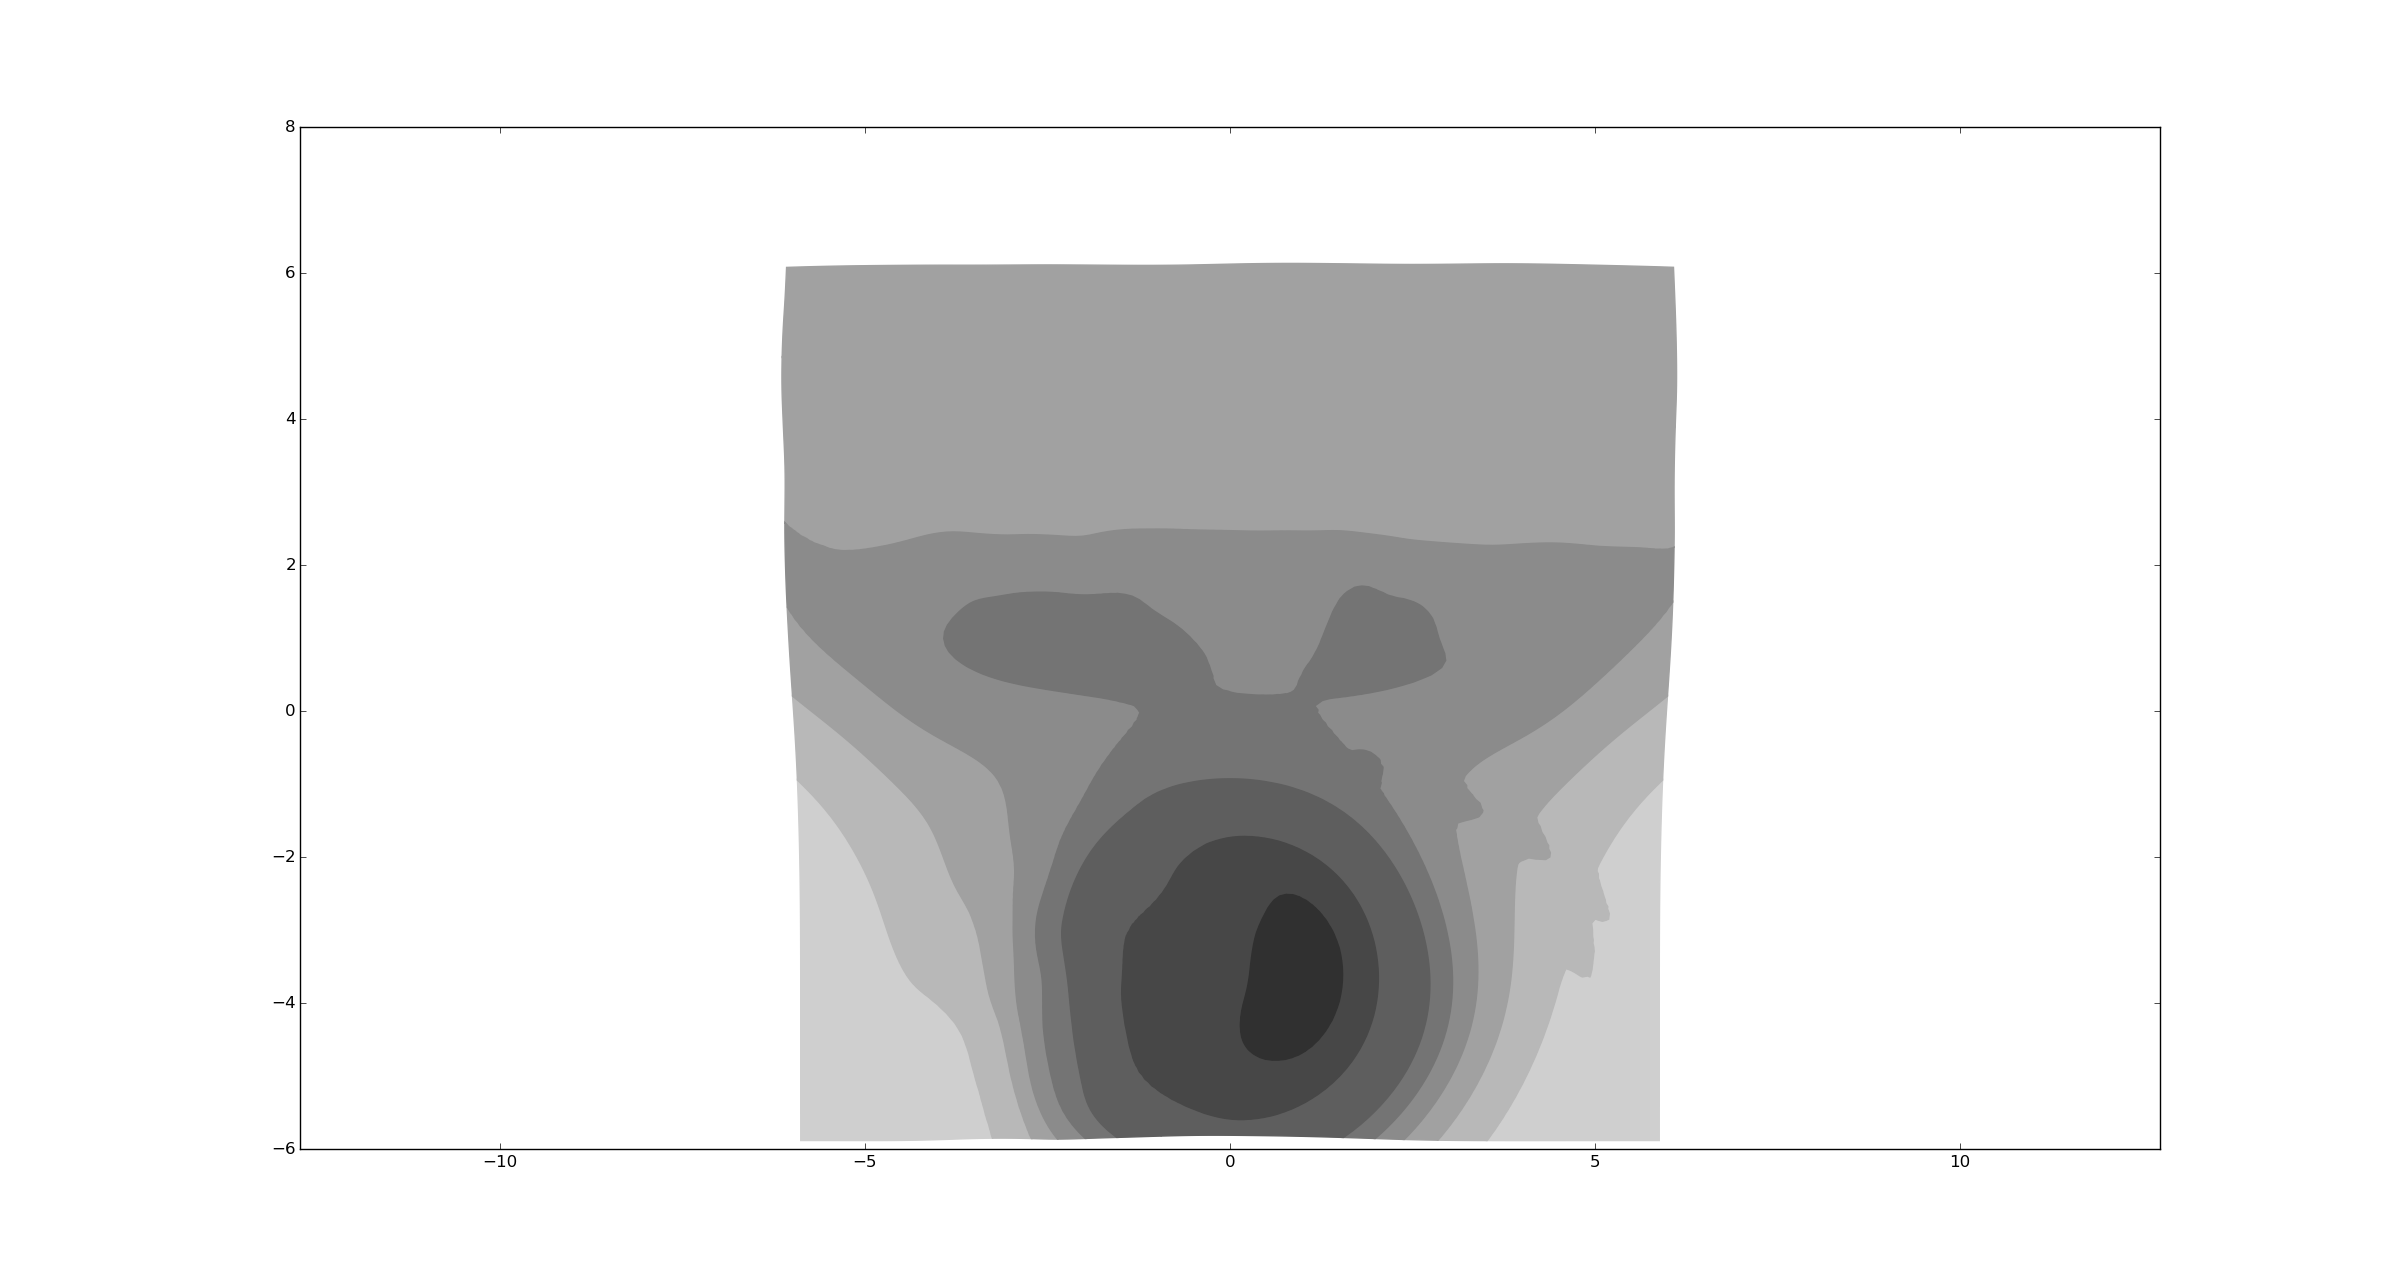
\includegraphics[scale=0.25]{big3.png}
        \caption{Результат работы программы. Модель 2, нижняя граница 0, верхняя граница 4.25, шаг 0.5.}
        \label{pic:big3}
    \end{figure}


    
    \clearpage


\section{Выводы}
    В рамках лабораторной работы были реализован алгоритм построения изоконтуров. Написана программа, позволяющая по модели строить горизонтальный разрез и визуализировать результаты. Из анализа результатов было получено: чем более крупный шаг мы выбираем, тем получаем менее подробную модель, но за меньшее время.
    
\end{document}